

\tikzset{every picture/.style={line width=0.75pt}} %set default line width to 0.75pt        

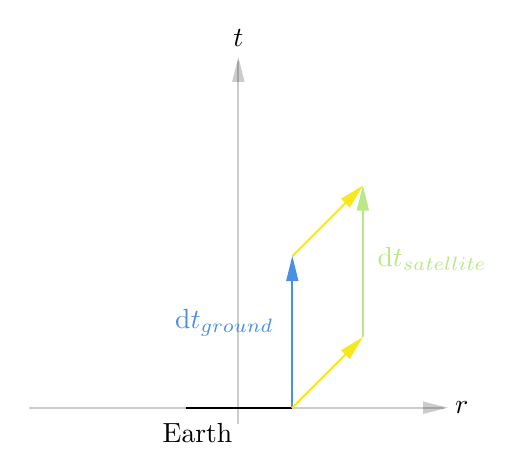
\begin{tikzpicture}[x=0.75pt,y=0.75pt,yscale=-1,xscale=1]
%uncomment if require: \path (0,300); %set diagram left start at 0, and has height of 300

%Straight Lines [id:da7136398117903702] 
\draw [color={rgb, 255:red, 0; green, 0; blue, 0 }  ,draw opacity=0.2 ]   (198,221) -- (398,221) ;
\draw [shift={(400,221)}, rotate = 180] [fill={rgb, 255:red, 0; green, 0; blue, 0 }  ,fill opacity=0.2 ][line width=0.08]  [draw opacity=0] (12,-3) -- (0,0) -- (12,3) -- cycle    ;
%Straight Lines [id:da6597324725387208] 
\draw [color={rgb, 255:red, 0; green, 0; blue, 0 }  ,draw opacity=0.2 ]   (299,229) -- (299,54) ;
\draw [shift={(299,52)}, rotate = 90] [fill={rgb, 255:red, 0; green, 0; blue, 0 }  ,fill opacity=0.2 ][line width=0.08]  [draw opacity=0] (12,-3) -- (0,0) -- (12,3) -- cycle    ;
%Straight Lines [id:da9825550559963256] 
\draw    (274,221) -- (325,221) ;
%Straight Lines [id:da031632983526935776] 
\draw [color={rgb, 255:red, 74; green, 144; blue, 226 }  ,draw opacity=1 ]   (325,150) -- (325,221) ;
\draw [shift={(325,148)}, rotate = 90] [fill={rgb, 255:red, 74; green, 144; blue, 226 }  ,fill opacity=1 ][line width=0.08]  [draw opacity=0] (12,-3) -- (0,0) -- (12,3) -- cycle    ;
%Straight Lines [id:da22827628675228628] 
\draw [color={rgb, 255:red, 248; green, 231; blue, 28 }  ,draw opacity=1 ]   (357.59,188.41) -- (325,221) ;
\draw [shift={(359,187)}, rotate = 135] [fill={rgb, 255:red, 248; green, 231; blue, 28 }  ,fill opacity=1 ][line width=0.08]  [draw opacity=0] (12,-3) -- (0,0) -- (12,3) -- cycle    ;
%Straight Lines [id:da6309512074381542] 
\draw [color={rgb, 255:red, 248; green, 231; blue, 28 }  ,draw opacity=1 ]   (357.59,115.41) -- (325,148) ;
\draw [shift={(359,114)}, rotate = 135] [fill={rgb, 255:red, 248; green, 231; blue, 28 }  ,fill opacity=1 ][line width=0.08]  [draw opacity=0] (12,-3) -- (0,0) -- (12,3) -- cycle    ;
%Straight Lines [id:da7011135365656176] 
\draw [color={rgb, 255:red, 184; green, 233; blue, 134 }  ,draw opacity=1 ]   (359,116) -- (359,187) ;
\draw [shift={(359,114)}, rotate = 90] [fill={rgb, 255:red, 184; green, 233; blue, 134 }  ,fill opacity=1 ][line width=0.08]  [draw opacity=0] (12,-3) -- (0,0) -- (12,3) -- cycle    ;

% Text Node
\draw (267.08,171.98) node [anchor=north west][inner sep=0.75pt]    {$\textcolor[rgb]{0.29,0.56,0.89}{\mathrm{d} t_{\text{ground}}}$};
% Text Node
\draw (364.58,141.98) node [anchor=north west][inner sep=0.75pt]  [color={rgb, 255:red, 184; green, 233; blue, 134 }  ,opacity=1 ]  {$\textcolor[rgb]{0.72,0.91,0.53}{\mathrm{d} t_{\text{satellite}}}$};
% Text Node
\draw (261,227) node [anchor=north west][inner sep=0.75pt]   [align=left] {Earth};
% Text Node
\draw (402,221) node [anchor=west] [inner sep=0.75pt]    {$r$};
% Text Node
\draw (299,48.6) node [anchor=south] [inner sep=0.75pt]    {$t$};


\end{tikzpicture}
